\documentclass[reqno, 12pt]{amsart}
\usepackage{enumerate}
\usepackage{amsmath}
\usepackage{scrextend}
\usepackage{bm}
\usepackage{algorithm}
\usepackage{algpseudocode}
\usepackage{graphicx}
\usepackage{enumitem}
\usepackage{tcolorbox}
\usepackage[headheight=12pt,textwidth=7in,top=1in, bottom=1in]{geometry}
\usepackage{listings}
\usepackage{cancel}
\usepackage{subcaption}
\usepackage{dirtree}
\usepackage{color} %red, green, blue, yellow, cyan, magenta, black, white
\definecolor{mygreen}{RGB}{28,172,0} % color values Red, Green, Blue
\definecolor{mylilas}{RGB}{170,55,241}

\usepackage[]{xcolor}
\definecolor{lightblue}{rgb}{0.63, 0.74, 0.78}
\definecolor{seagreen}{rgb}{0.18, 0.42, 0.41}
\definecolor{orange}{rgb}{0.85, 0.55, 0.13}
\definecolor{silver}{rgb}{0.69, 0.67, 0.66}
\definecolor{rust}{rgb}{0.72, 0.26, 0.06}
\definecolor{purp}{RGB}{68, 14, 156}

\colorlet{lightrust}{rust!50!white}
\colorlet{lightorange}{orange!25!white}
\colorlet{lightlightblue}{lightblue}
\colorlet{lightsilver}{silver!30!white}
\colorlet{darkorange}{orange!75!black}
\colorlet{darksilver}{silver!65!black}
\colorlet{darklightblue}{lightblue!65!black}
\colorlet{darkrust}{rust!85!black}
\colorlet{darkseagreen}{seagreen!85!black}

\usepackage{hyperref}
\hypersetup{
  colorlinks=true,
}

\hypersetup{
  linkcolor=darkrust,
  citecolor=seagreen,
  urlcolor=darkrust,
  pdfauthor=author,
}

\usepackage{cleveref}

%some custom commands you may find useful
\usepackage{xparse}
\DeclareDocumentCommand{\diff}{O{} m}{
	\frac{\mathrm{d} #1}{\mathrm{d}#2}
}
\DeclareDocumentCommand{\difftwo}{O{} m}{
	\frac{\mathrm{d}^2 #1}{\mathrm{d}#2^2}
}
\DeclareDocumentCommand{\pdiff}{O{} m}{
	\frac{\partial #1}{\partial #2}
}
\DeclareDocumentCommand{\pdifftwo}{O{} m}{
	\frac{\partial^{2} #1}{\partial #2^{2}}
}
\DeclareDocumentCommand{\integral}{O{} O{} m O{x}}{
	\int_{#1}^{#2} #3\ \mathrm{d}#4
}
\DeclareDocumentCommand{\sp}{}{
	\qquad \qquad \qquad }{
}
\NewDocumentEnvironment{solution}{}{
	\begin{addmargin}[2em]{0pt}
	}{\end{addmargin} \vskip0.25cm
}

\newenvironment{sysmatrix}[1]
{\left(\begin{array}{@{}#1@{}}}
	{\end{array}\right)}
\newcommand{\ro}[1]{%
	\xrightarrow{\mathmakebox[\rowidth]{#1}}%
}
\newlength{\rowidth}% row operation width
\AtBeginDocument{\setlength{\rowidth}{3em}}

\def\name{Ben Wilfong} %your name goes here
\def\ID{bwilfong3} %your cm goes here

%these packages create the footer and page numbering
\usepackage{fancyhdr}
\usepackage{lastpage}
\pagestyle{fancy}
\lhead{\name}
%%%%%%%%%%%%%%%%%%%%%%%%%%%%%%%%
\chead{ME 7751 Homework \#3}
%%%%%%%%%%%%%%%%%%%%%%%%%%%%%%%%
\rhead{Username: \ID}
\fancyfoot[C]{\footnotesize Page \thepage\ of \pageref{LastPage}}
\fancypagestyle{firststyle}
{ \renewcommand{\headrulewidth}{0pt}%
	\fancyhf{}%
	\fancyfoot[C]{\footnotesize Page \thepage\ of \pageref{LastPage}}
}

\lstset{frame=tb,
  language=[90]Fortran,
  aboveskip=3mm,
  belowskip=3mm,
  showstringspaces=false,
  columns=flexible,
  basicstyle={\footnotesize\ttfamily},
  numbers=none,
  numberstyle=\tiny\color{gray},
  keywordstyle=\color{darklightblue},
  commentstyle=\color{seagreen},
  stringstyle=\color{darkrust},
  breaklines=true,
  breakatwhitespace=true,
  tabsize=3,
}

\begin{document}
	\noindent
	\thispagestyle{firststyle}
	%\begin{tabular}{l}
		%{\LARGE \textbf{ME 7751: Intro to CFD} }\\
		%%%%%%%%%%%%%%%%%%%%%%%%%%
		%{\Large Homework Set \#1}
		%%%%%%%%%%%%%%%%%%%%%%%%%%
	%\end{tabular} \hfill \begin{tabular}{r}
		%\name \\
		%Username: \ID
	%\end{tabular}
	%\noindent\makebox[\linewidth]{\rule{\textwidth}{1pt}}

    \begin{center}
        \LARGE{\textbf{Solution of the 1D unsteady transport equation with the finite difference method}} \\
        \Large{October 16$^{th}$, 2024} \\
        \large{Ben Wilfong}
    \end{center}
    \section*{Files}
    \dirtree{%
         .1 HW3\_root.
         .2 CMakeLists.txt.
         .2 homework.pdf.
         .2 main.inp.
         .2 make.sh.
         .2 src.
         .3 m\_global\_parameters.f90.
         .3 m\_helpers.f90.
         .3 m\_linear\_algebra.f90.
         .3 p\_main.f90.
         .2 plots.
         .3 *.csv.
         .3 plots.m.
    }
    \section*{Compiling}
    \noindent This code can be compiled in a terminal by running \texttt{chmod u+x ./make.sh} followed by \texttt{./make.sh} in the \texttt{HW3\_root/} directory.
    This will compile and link the source code in the \texttt{src/} directory and create an executable called \texttt{main} in the \texttt{HW3\_root/} directory.
    \section*{Running}
    \noindent The problem parameters are defined in the namelist file \texttt{main.inp} in \texttt{HW3\_root/}.
    The input parameters are:
    \begin{itemize}
        \setlength\itemsep{-0.1em}
        \item gamma: Difusion coefficient
        \item U: advection speed
        \item bench: logical enabling multiple runs of the code for benchmarking runtime
        \item time\_stepper: which time-stepper to use. 0 = Explicit Euler, 1 = Implicit Euler, 2 = Crank-Nicolson
        \item N: number of points
        \item dt: time-step
        \item t\_start: start time
        \item t\_stop: end time
        \item t\_save: time interval between saves
    \end{itemize}
    Once the input parameters are set, the code is ran with \texttt{./main}.
    After execution, the solution is written to \texttt{HW3\_root/output.csv} with the first row holding the x coordinates and each following row storing $\phi$ at a different instance in time.    \newpage

    \section*{Part 1: Numerical Schemes}
    \noindent The one-dimensional unsteady transport equation can be written with time-derivatives on the LHS and spatial derivatives on the RHS as
    \begin{equation*}
        \pdiff[\phi]{t} = \pdiff{x}\left(\Gamma\pdiff[\phi]{x}\right) - U\pdiff[\phi]{x}.
    \end{equation*}
    For the case of constant $U$ and $\Gamma$, the above simplifies to
    \begin{equation*}
        \qquad \pdiff[\phi]{t} = f(\phi) \text{ where } f(\phi) = \Gamma\pdifftwo[\phi]{x} - U\pdiff[\phi]{x}.
    \end{equation*}
    $f(\phi^{(n)})$ can be discretized using central differences as
    \begin{align*}
        f(\phi^{(n)}_i) &=
                        \Gamma\frac{\phi^{(n)}_{i + 1} - 2\phi^{(n)}_i + \phi^{(n)}_{i - 1}}{\left(\Delta x\right)^2} -
                        U\frac{\phi^{(n)}_{i + 1} - \phi^{(n)}_{i - 1}}{2\Delta x}, \\
                        &= \left(\frac{\Gamma}{\left(\Delta x\right)^2} - \frac{U}{2\Delta x}\right)\phi^{(n)}_{i + 1} +
                        \left(-\frac{2\Gamma}{\left(\Delta x\right)^2}\right)\phi^{(n)}_{i} +
                        \left(\frac{\Gamma}{\left(\Delta x\right)^2} + \frac{U}{2\Delta x}\right)\phi^{(n)}_{i - 1}.
    \end{align*}
    This discretization can be used to formulate temporal integration schemes using forward Euler, backward Euler, and Crank--Nicolson methods with the diffusion and Courant numbers
    \begin{equation*}
        d = \frac{\Gamma \Delta t}{\left(\Delta x\right)^2} \quad \text{and} \quad c = \frac{U\Delta t}{\Delta x}
    \end{equation*}
    as follows:
    \begin{itemize}
        \item \textbf{Forward Euler} defines the solution at $t^{(n+1)}$ as $\phi^{(n+1)} = \phi^{n} + \Delta t f(\phi^{(n)},t^n)$.
        Using the above discretization of $f(\phi^{(n)})$ gives the explicit update equation
        \begin{equation*}
            \phi_{i}^{(n+1)} = \left(d + \frac{c}{2}\right)\phi_{i-1}^{(n)} + \left(1 - 2d\right)\phi_i^{(n)} + \left(d - \frac{c}{2}\right)\phi_{i + 1}^{(n)}.
        \end{equation*}
        This explicit update, after taking into account boundary conditions, can be written as the tridiagonal matrix multiplication
        \begin{equation*}
            \underbrace{
            \begin{pmatrix}
                \phi_0^{(n+1)} \\ 
                \phi_1^{(n+1)} \\ 
                \vdots \\ 
                \phi_{N-1}^{(n+1)} \\ 
                \phi_N^{(n+1)}
            \end{pmatrix}}_{\Phi^{(n+1)}}
            =
            \underbrace{
            \begin{pmatrix}
                0 & 0 & 0 \\ 
                d + c/2 & 1 - 2d & d - c/2 \\
                \hfill \ddots & \hfill \ddots & \hfill \ddots \\
                & d + c/2 & 1 - 2d & d - c/2 \\
                & 0 & 0 & 0
            \end{pmatrix}
            \begin{pmatrix}
                \phi_0^{(n)} \\ 
                \phi_1^{(n)} \\ 
                \vdots \\ 
                \phi_{N-1}^{(n)} \\ 
                \phi_N^{(n)}
            \end{pmatrix}}_{\text{RHS}}.
        \end{equation*}
    \item \textbf{Backward Euler} defines the solution at $t^{(n+1)}$ as $\phi^{(n+1)} = \phi^{(n)} + \Delta t f(\phi^{(n+1)}, t^{n+1})$.
        Using the above discretization of $f(\phi^{(n)})$ gives the implicit update equation
        \begin{equation*}
            \left(-\frac{c}{2}-d\right)\phi^{(n+1)}_{i-1} + \left(1 + 2d\right)\phi^{(n+1)}_i + \left(\frac{c}{2} - d\right)\phi^{(n+1)}_{i + 1} = \phi^{(n)}_i.
        \end{equation*}
        This implicit update equation, after taking into account boundary conditions, can be written as the tridiagonal system of linear equations
        \begin{equation*}
            \underbrace{
            \begin{pmatrix}
                1 & 0 & 0 \\
                -c/2 - d & 1 + 2d & c/2 - d \\
                \hfill \ddots & \hfill \ddots & \hfill \ddots \\
                & -c/2 - d & 1 + 2d & c/2 - d \\
                & 0 & 0 & 1
            \end{pmatrix}}_{A}
            \underbrace{
            \begin{pmatrix}
                \phi_0^{(n+1)} \\
                \phi_1^{(n+1)} \\ 
                \vdots \\
                \phi_{N-1}^{(n+1)} \\
                \phi_{N}^{(n+1)}
        \end{pmatrix}}_{\Phi^{(n+1)}}
            =
            \underbrace{
            \begin{pmatrix}
                0 \\
                \phi_1^{(n+1)} \\ 
                \vdots \\
                \phi_{N-1}^{(n+1)} \\
                0
        \end{pmatrix}}_{\text{RHS}}
        \end{equation*}
    \item \textbf{Crank--Nicolson} defines the solution at $t^{(n+1)}$ as
        \[\phi^{(n+1)} = \phi^{(n)} + (\Delta t)/2\left(f(\phi^{(n+1)},t^{(n+1)}) + f(\phi^{(n)}, t^{(n)})\right).\]
        Using the discretization of $f(\phi^{(n)})$ gives the implicit--explicit update equation
        \begin{align*}
            \left(-\frac{c}{4}-\frac{d}{2}\right)\phi^{(n+1)}_{i-1} &+ \left(1 + d\right)\phi^{(n+1)}_i + \left(\frac{c}{4} - \frac{d}{2}\right)\phi^{(n+1)}_{i + 1} = \dots\\
            & \left(\frac{d}{2} + \frac{c}{4}\right)\phi_{i-1}^{(n)} + \left(1 - d\right)\phi_i^{(n)} + \left(\frac{d}{2} - \frac{c}{4}\right)\phi_{i + 1}^{(n)}.
        \end{align*}
        This implicit--explicit update equation, after taking into account boundary conditions, can be written as the tridiagonal system of linear equations
        \begin{align*}
            &\underbrace{
            \begin{pmatrix}
                1 & 0 & 0 \\
                -c/4 - d/2 & 1 + d & c/4 - d/2 \\
                \hfill \ddots & \hfill \ddots & \hfill \ddots \\
                & -c/4 - d/2 & 1 + d & c/4 - d/2 \\
                & 0 & 0 & 1
            \end{pmatrix}}_{A}
            \underbrace{
            \begin{pmatrix}
                \phi_0^{(n+1)} \\
                \phi_1^{(n+1)} \\ 
                \vdots \\
                \phi_{N-1}^{(n+1)} \\
                \phi_{N}^{(n+1)}
            \end{pmatrix}}_{\Phi^{(n+1)}}
                =\\
            &\qquad\qquad\qquad\qquad\underbrace{
            \begin{pmatrix}
                0 & 0 & 0 \\ 
                d/2 + c/4 & 1 - d & d/2 - c/4 \\
                \hfill \ddots & \hfill \ddots & \hfill \ddots \\
                & d/2 + c/4 & 1 - d & d/2 - c/4 \\
                & 0 & 0 & 0
            \end{pmatrix}
            \begin{pmatrix}
                \phi_0^{(n)} \\ 
                \phi_1^{(n)} \\ 
                \vdots \\ 
                \phi_{N-1}^{(n)} \\ 
                \phi_N^{(n)}
            \end{pmatrix}}_{\text{RHS}}.
        \end{align*}
    \end{itemize}

    \section*{Part 2: Problem 2}
    \noindent \Cref{fig:comp} shows the solution using all three methods at $T = 20, 30$ and $40$ in the first three rows.
    The first column shows a zoomed in view of the peak of the solution to highlight the minor differences between the three methods for case 1, which is shown in the second column.
    The solution for case 2 is given in the third column.
    The solutions to case 2 have spurious oscillations for all three temporal integrators.
    This is becuse there is no diffusion to damp these oscillations.
    The figure in the fourth row shows the soltuion at $T = 10, 20, 30,$ and $40$ for case 1 using Crank--Nicolson for time integration.
    The diffusion causes the signal's height to decrease while its' width increases.
    $N = 500$ was used for all solutions in this figure.
    \begin{figure}
        \centering
        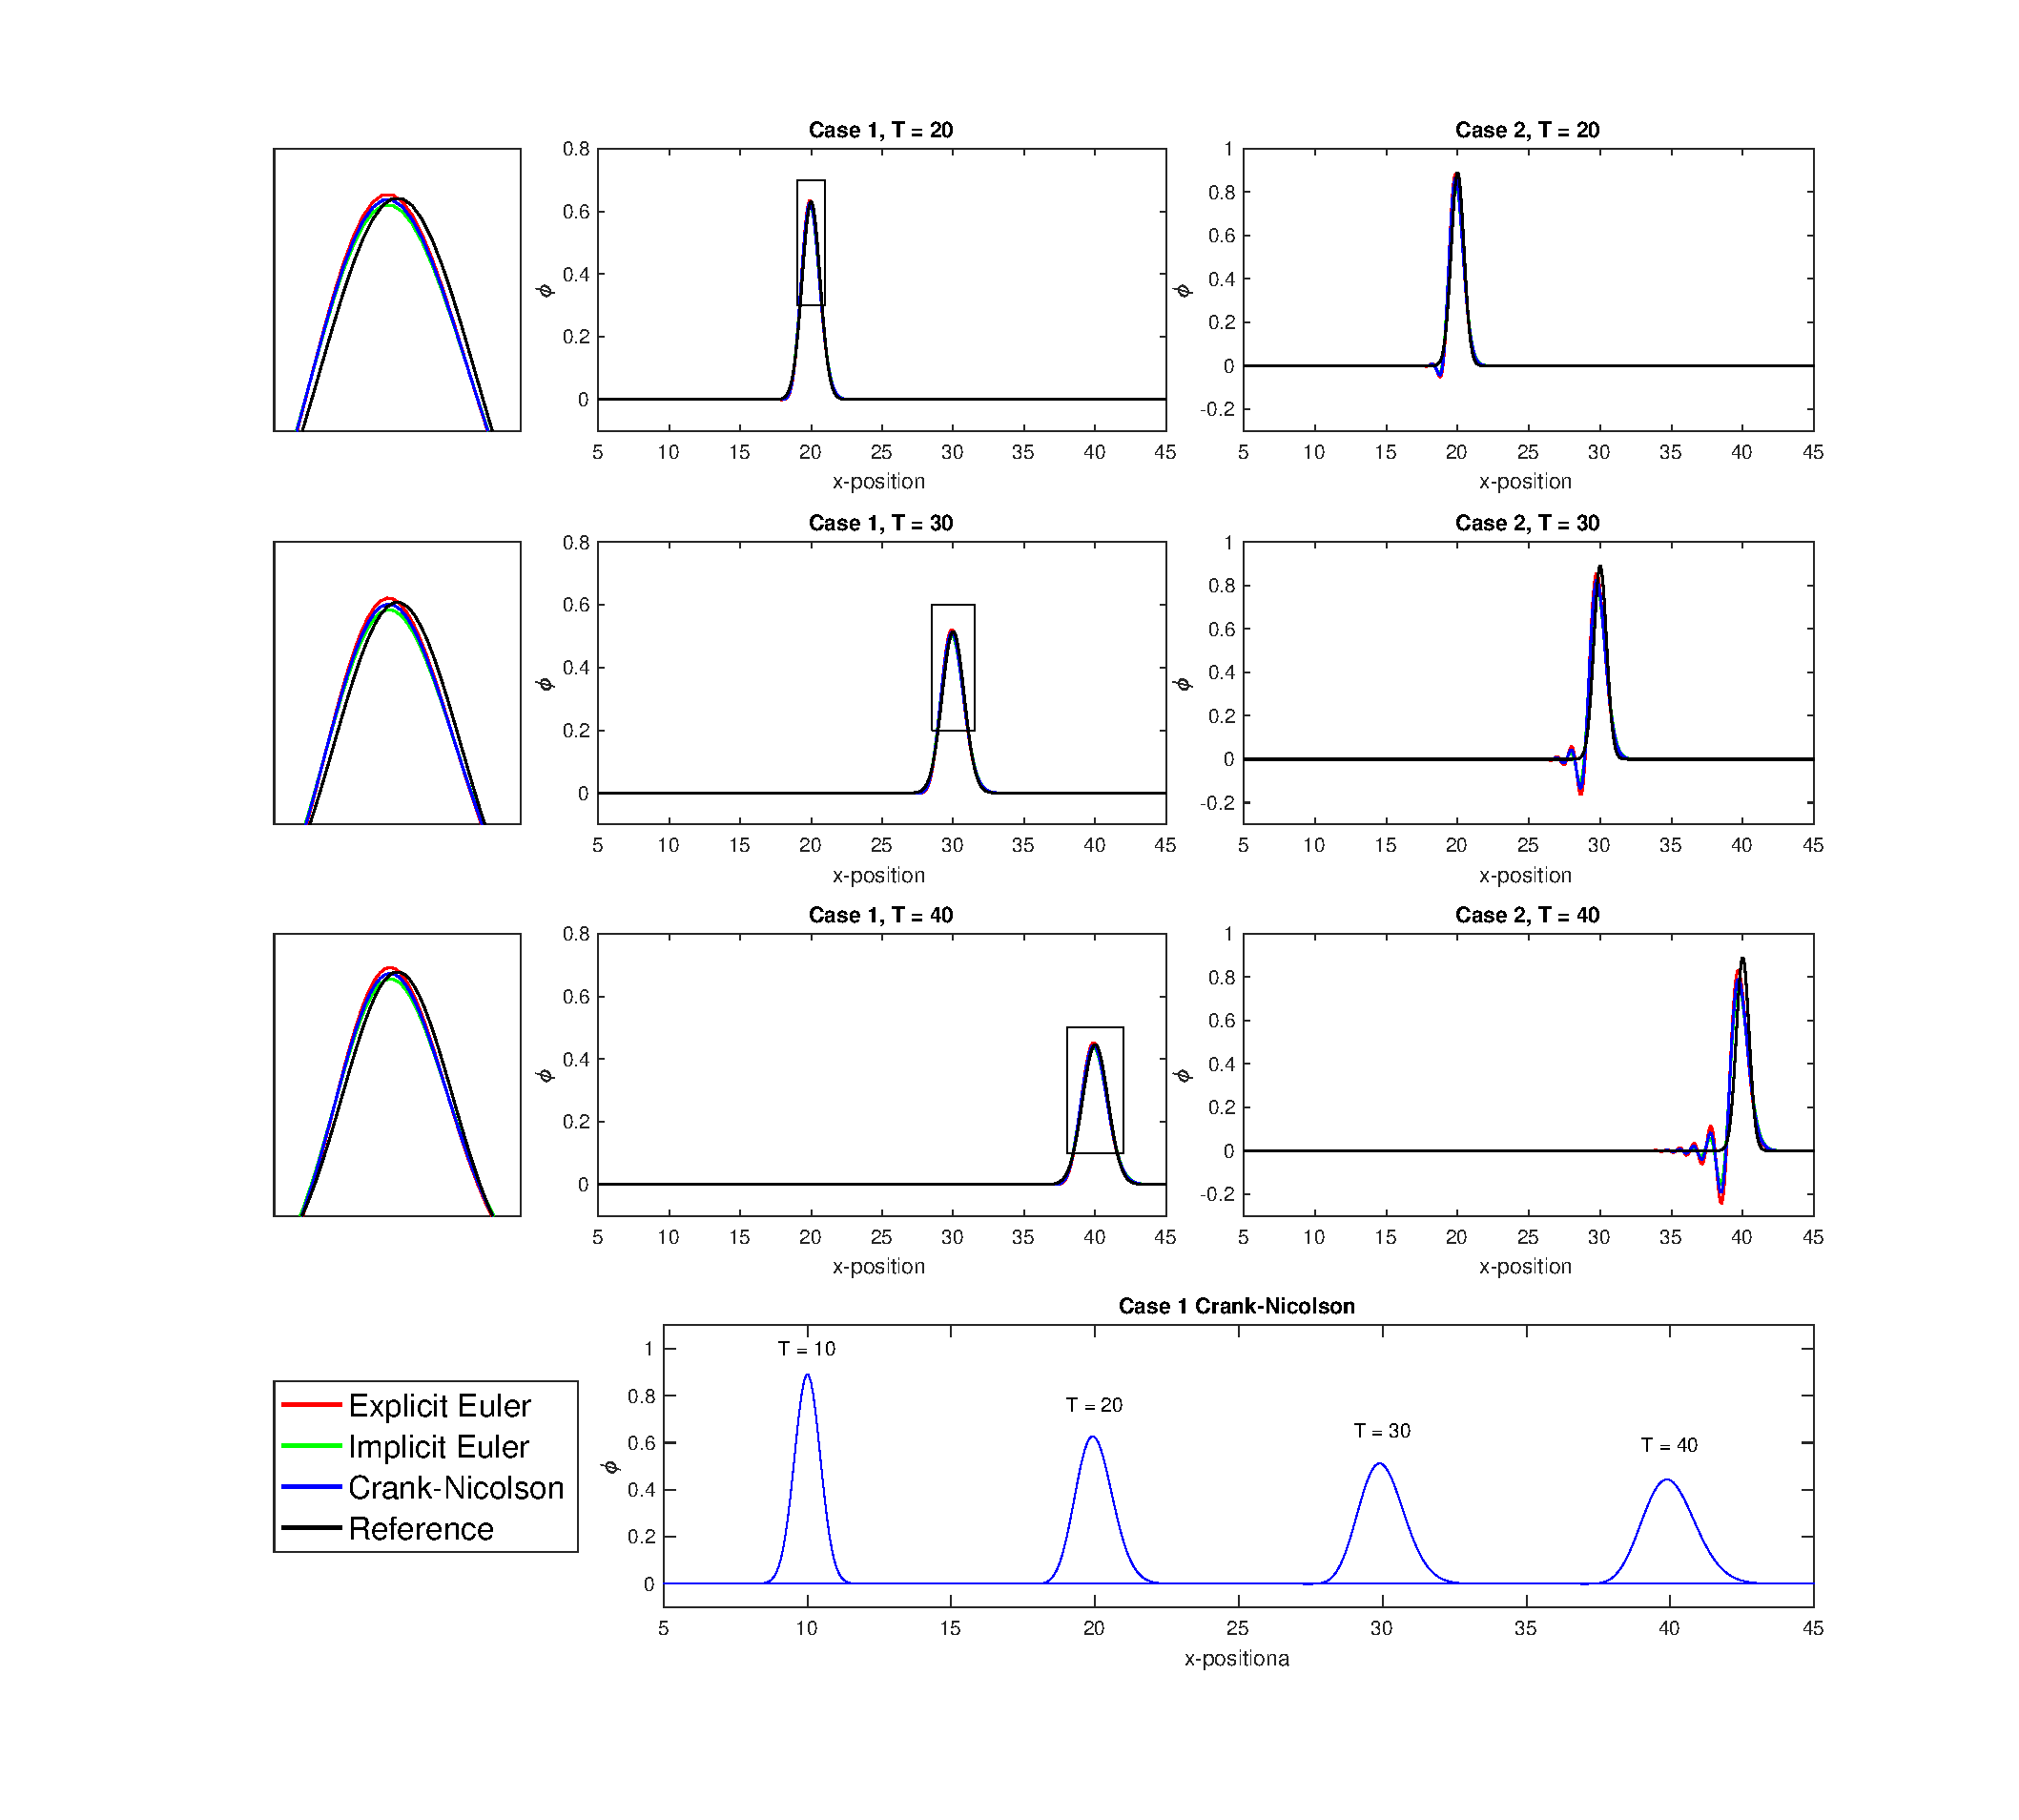
\includegraphics[width=\textwidth]{P2.eps}
        \caption{Comparision of the three numerical schemes}
        \label{fig:comp}
    \end{figure}

    \section*{Part 3: Problem 3}
    \noindent \Cref{fig:phiT} shows the value of $\phi$ as a function time at $x =  15$ and $x = 25$ for the three numerical methods.
    Explcit Euler overshoots the reference solution while implicit Euler undershoots the reference solution.
    Crank--Nicolson shows the best agreement of the three because it is essentially an average of implicit and explicit Euler.
    \begin{figure}
        \centering
        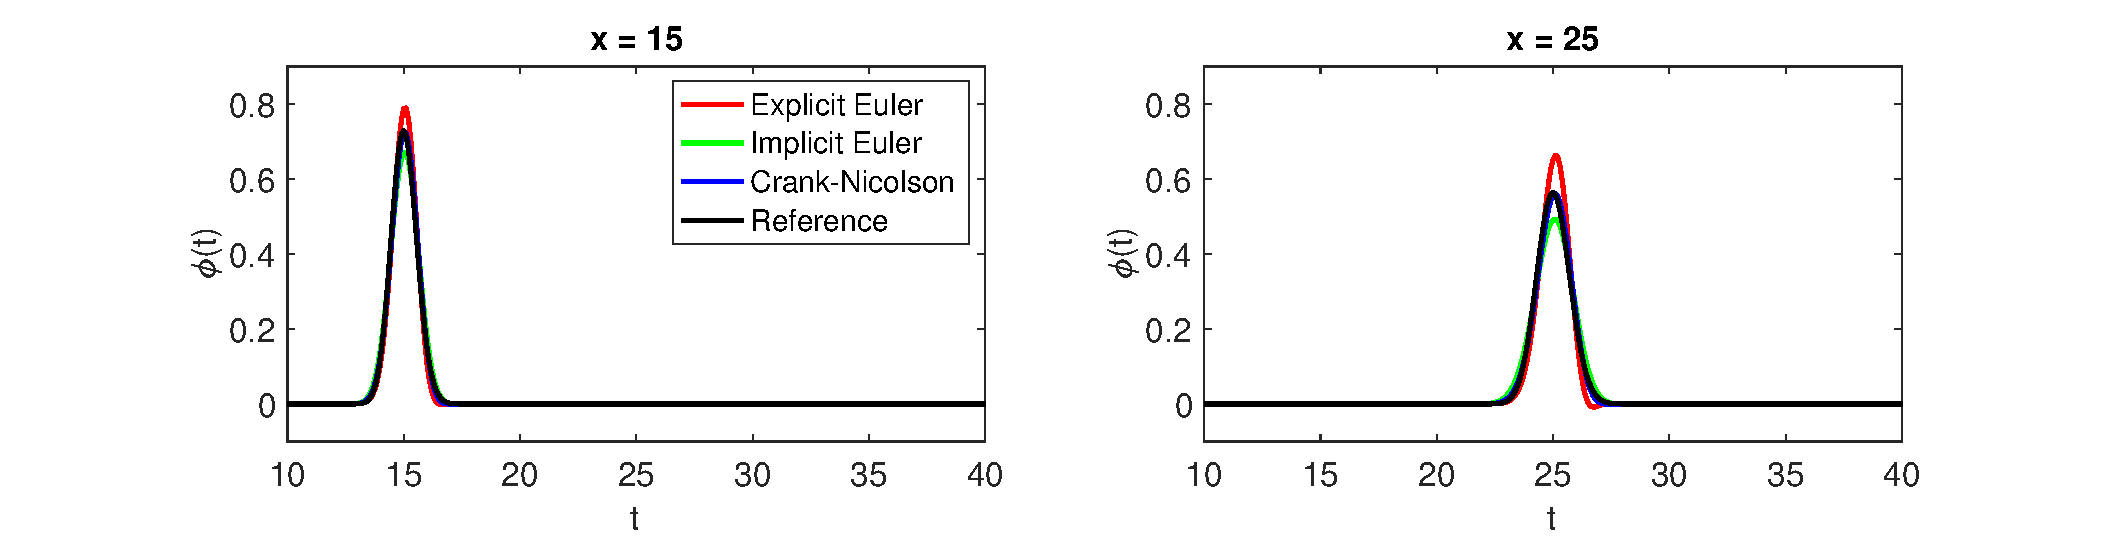
\includegraphics[width=\textwidth]{P3.eps}
        \caption{$\phi(t)$ at $x = 15$ and $x = 25$}
        \label{fig:phiT}
    \end{figure}

    \section*{Part 4: Spatial Convergence}
    \noindent \Cref{fig:spatConv} shows the spatial convergence of Crank-Nicolson.
    The emperical spatial convergence rate is second order, which agrees with the second order central difference scheme used to discretize the spatial derivatives.
    \begin{figure}
        \centering
        \begin{subfigure}[t]{0.4\textwidth}
            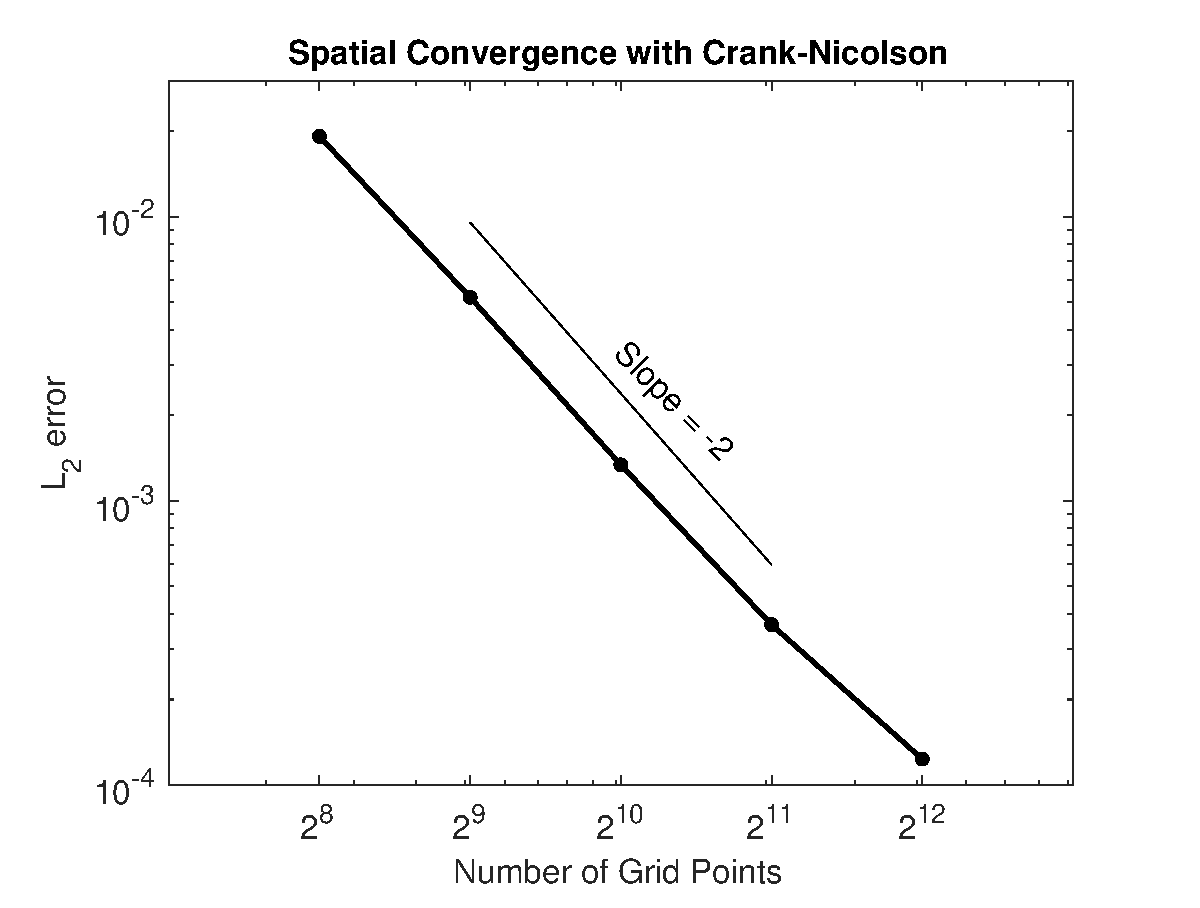
\includegraphics[width=\textwidth]{P4.eps}
            \caption{Spatial Convergence}
            \label{fig:spatConv}
        \end{subfigure}
        \begin{subfigure}[t]{0.4\textwidth}
            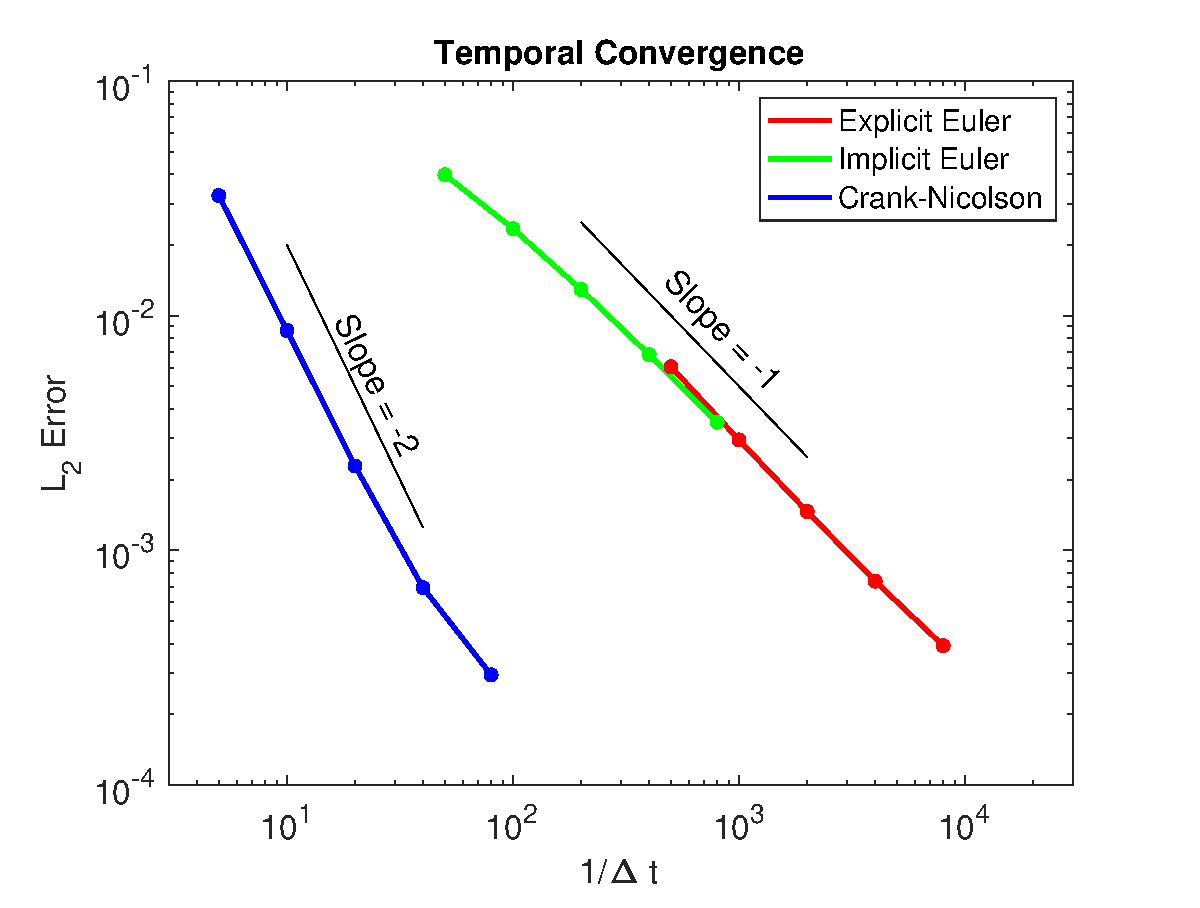
\includegraphics[width=\textwidth]{P5.eps}
            \caption{Temporal Convergence}
            \label{fig:tempConv}
        \end{subfigure}
        \caption{Convergence}
    \end{figure}

    \section*{Part 5: Temporal Convergence}
    \noindent \Cref{fig:tempConv} shows the temporal convergence of of all three time integegrators for $N = 4096$.
    Implicit and Explicit Euler both show first order accuracy in time while Crank--Nicolson exhibits second order accuracy in time.
    Larger time-steps were used for Crank-Nicolson to ensure that the temporal accuracy was being measured rather than the spatial accuracy.
    As the time-step decreases, the temporal convergence flatlines as spatial discretization error becomes dominant.

    \section*{Part 6: Stability}
    \noindent Explicit Euler is conditionally stable when used to solve the 1D unsteady transport equation while Implicit Euler and Crank-Nicolson are unconditionally stable due to their implicit nature.
The stability criterion for explicit Euler can be calculated using Von Neumann stability analysis by substituting the Fourier modes $\phi_j^{(n)} = e^{ij\Delta x\xi}$ and $\phi_j^{(n+1)} = g(\xi)e^{ij\Delta x\xi}$ into the update equation, which gives
    \begin{equation*}
        g(\xi)e^{ij\Delta x\xi} = \left(d + \frac{c}{2}\right)e^{i(j-1)\Delta x\xi} + \left(1 - 2d\right)e^{ij\Delta x\xi} + \left(d - \frac{c}{2}\right)e^{i(j+1)\Delta x\xi}.
    \end{equation*}
    Dividing each side by $e^{ij\Delta x\xi}$ and simplifying gives
    \begin{align*}
        g(\xi) &= \left(d + \frac{c}{2}\right)e^{-i\Delta x\xi} + \left(1 - 2d\right) + \left(d - \frac{c}{2}\right)e^{i\Delta x\xi}, \\
        g(\xi) &= \left(d + \frac{c}{2}\right)\left(\cos(\xi\Delta x) - i\sin(\xi\Delta x)\right) + \left(1 - 2d\right) + \left(d - \frac{c}{2}\right)\left(\cos(\xi\Delta x) + i\sin(\xi\Delta x)\right), \\
        g(\xi) &= 1 + 2d\left(\cos(\xi\Delta x) - 1\right) + c\sin(\xi\Delta x).
    \end{align*}
    If there is no diffusion, then $d = 0$ and $|g(\xi)| \ge 1$ for all $\Delta t$ mean the method is unconditinally unstable without difussion.
    If there is no convection, then the method is stable when $d < 1/2,$ which gives the constraint $\Delta t < (\Delta x)^2/(2\Gamma)$.
    If $d \ne 0$ and the problem is dominated by convection, then $\Delta t < \Delta x/U$ must be satisfied.

    \section*{Part 7: Runtime}
    \noindent Figure 4 shows the time to solution and time per time-step for each numerical method for a fixed $\Delta t$.
    \Cref{tab:runtime} shows the exact runtime per time-step for each numerical method.
    All three time integrators show $\mathcal{O}(n)$ runtime as expected.
    Crank--Nicolson and Implicit Euler both take significantly longer due to the implicit solve required at each time-step.
    This implicit solve provides more value when using Crank--Nicolson because it greatly reduces temporal discretization error as shown in \Cref{fig:tempConv}.
    This reduction in temporal discretization error ultimately means that fewer timesteps are required than for explicit Euler, meaning that the time to solution for the same target accuracy is actually less for Crank--Nicolson than for explicit Euler as a result of its higher order temporal accuracy.
    \begin{figure}
        \centering
            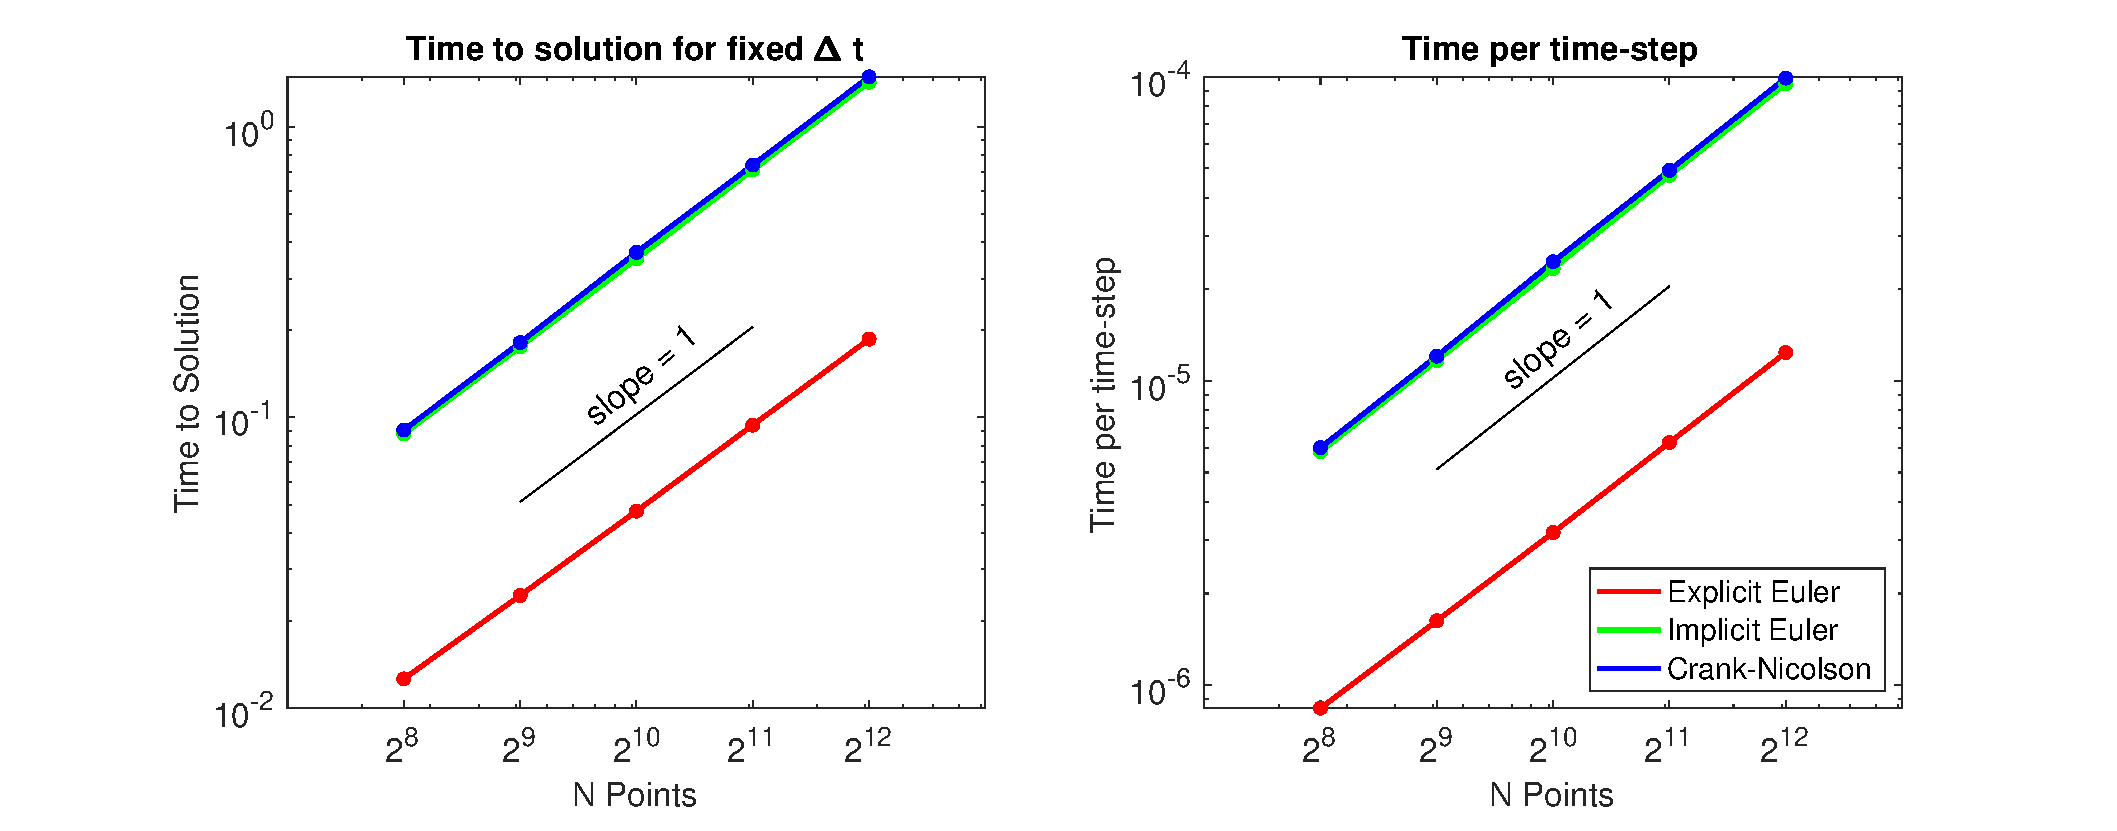
\includegraphics[width=0.8\textwidth]{P7.eps}
            \label{fig:runtime}
            \caption{Time to solution and time per time-step for fixed $\Delta t$}
    \end{figure}
    \begin{table}
        \caption{Time per time-step for each numerical method in $\mu$s}
        \begin{tabular}{ c | c c c}
            \hline N & Explicit Euler & Implicit Euler & Crank--Nicolson \\ \hline
            256 & 0.84 & 5.85 & 6.03 \\
            512 & 1.62 & 11.7 & 12.1\\
            1024 & 3.17 & 23.4 & 24.7\\
            2048 & 6.27 & 47.4 & 49.3\\
            4096 & 12.4 & 94.9 & 99.1\\ \hline
        \end{tabular}
        \label{tab:runtime}
    \end{table}


\end{document}

